\chapter{Emulation and Monitoring of the Upstream Tracker RAW data}

This chapter is dedicated to present the TbUT, the tool that was designed to emulate all raw data processing algorithms. This software was implemented in order to process a raw data collected during the UT testbeams and it will play a crucial role in the future monitoring and calibration of the UT detector. 

The crucial and first test to this software was UT testbeams, where TbUT was used as the main software to decode and process all collected data. The next sessions present a detailed description of each of the processing steps.


\section{TbUT Emulation Software}
\label{chapter:tbut}
The TbUT package is a software developed entirely by the author and it is based on the Gaudi framework \cite{Gaudi}. Gaudi identifies components with specific purposes and well defined interfaces, interacting with each other to provide the whole functionality of an application. Gaudi provides to the application general purpose components, like messaging and configuration services, see figure \ref{fig:gaudi flow}. The configuration is performed via the customized python scripts. By design, the Gaudi framework decouples objects describing data from those describing algorithms.



\begin{figure}[h]
\centering
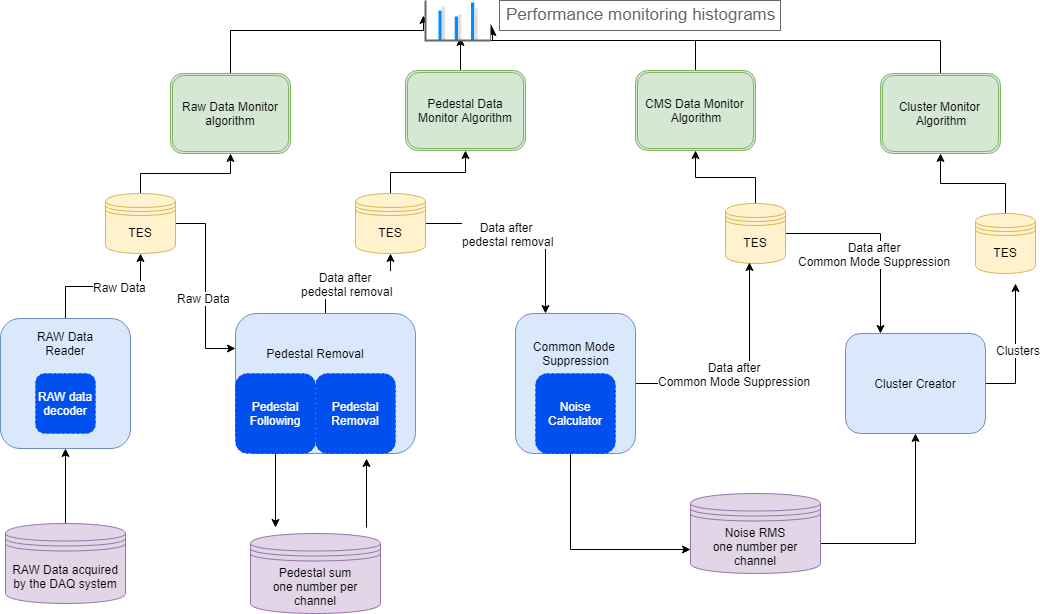
\includegraphics{figures/TBUT.png}
\caption{The diagram presenting the main component of the TbUT package and interactions between them. The light blue components are algorithms, dark blue are tools, and the violet ones represents serializable data. The direction of the arrows indicates whether the data is an input or output to the algorithm. }
\label{fig:TbUT}
\end{figure}

It allows performing full UT DUT data processing.
The software was designed based on the Objected Oriented Programming paradigm and each of the component inherit from one the following classes:  

\begin{itemize}
    \item \textbf{Algorithms}, these objects inherit from \textit{Gaudi::algorithm}, which is an essential part of the Gaudi application. They can read the input data, and via an appropriate tool process, they are able to generate the monitoring plots and store the data for the next processing steps. 
    \item \textbf{Monitoring algorithm}, these object, similarly to the \textbf{Algorithms}, inherit from  \textit{Gaudi::algorithm}. Their job is to extract data from TES and generate a set of monitoring histograms, which suppose to give an  ultimate answer on the performance of the sensor. This component is a key to make a  proper calibration. 
    \item \textbf{Tools} These objects inherit from the pure virtual interface \textit{IProcessingEngine} and they were designed to perform the processing actions, for instance, pedestal removal. Figure \ref{fig:gaudi flow} presents the main components of the Gaudi framework.   
    \item \textbf{Serializable data} this objects inherits from the \textit{GaudiKernel::DataObject} are the result of the processing via the \textbf{Tools} and can be stored inside the Transient Event Store (TES). 
    \item \textbf{Tool's Factories} this types of objects were implemented to dynamically create tools. Its concept was introduced in the Design Pattern book \cite{DesignPatterns}. 
\end{itemize}

\begin{figure}[h]
\centering
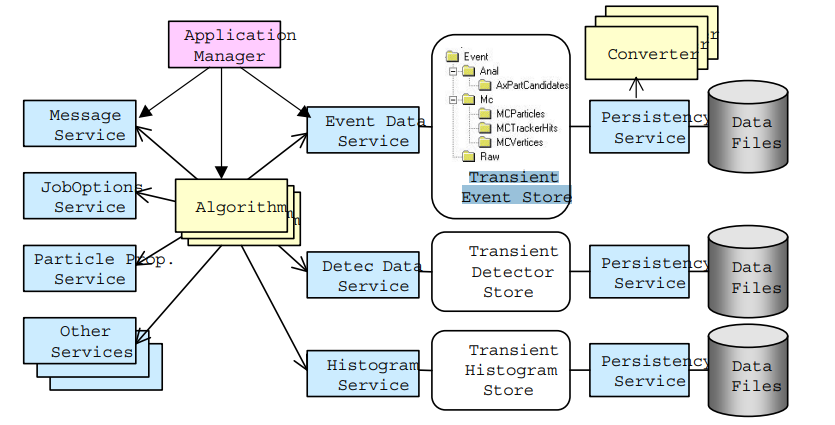
\includegraphics{figures/Gaudi.png}
\caption{Object Diagram of the GAUDI Architecture, figure taken from \cite{Gaudi}}
\label{fig:gaudi flow}
\end{figure}


The first algorithm within the TbUT is dedicated to decoding the raw data acquired by the acquisition board, which is visualized in figure \ref{fig:TbUT}.  
During the lifetime of this project, the software has to able to process data acquired by the number of different DAQ systems, each of these producing the data in a completely different format.  To achieve that kind of flexibility the tool, that is responsible for reading the input data was implemented using a Factory Design Pattern \cite{DesignPatterns}. 

\subsection{Pedestal Subtraction}

Pedestals are the charge values measured by the read-out system in the absence of signal and noise. Each of the read-out channels can have a different ADC value of pedestal and the value of each pedestal depends on such environmental conditions as temperature and humidity as well as operating conditions, like applied bias voltage. 
To ensure that proper pedestals are removed from the raw ADC data, prior to each data collection run the non-signal measurements (pedestal runs) ware taken. 

The pedestal subtraction algorithm has two phases. In first, the pedestal values are calculated. During the second one the determined pedestal values are subtracted from the raw ADC data. Figure \ref{fig:ped} presents Pedestal Subtraction algorithm sequence diagram. That kind of UML diagram \cite{UML} is dedicated to depicts interaction between objects in a sequential order. These diagrams are widely used by businessmen and software developers to document and understand requirements for new and existing systems. 

\begin{figure}
\centering
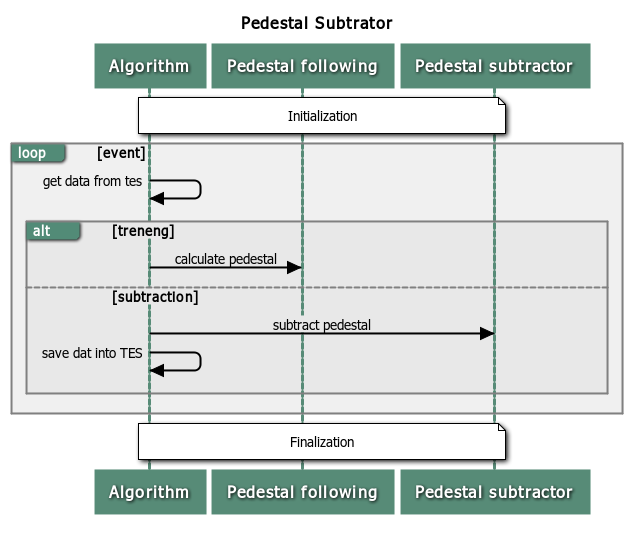
\includegraphics[scale=0.6]{figures/Pedestal_Subtrator.png}
\caption{Pedestal Subtraction sequence diagram.}
\label{fig:ped}
\end{figure}



\subsubsection{Pedestal following}
From the mathematical point of view the calculation of the pedestal is a running average. In every training event then pedestal sum is updated. This update takes into account the previously calculated value of the pedestal sum and the current ADC count. The pedestal sum is calculated for each channel separately. To be more precisely, the pedestal sum, $p^{sum}_i(n)$, for channel $i$ and event $n$ can be expressed as follows:

\begin{equation}
P_{i}^{sum}(n+1)=P^{sum}_{i}(n) + \frac{\Delta_{i}(n+1)}{N}
\label{eq:ped}
\end{equation}
Where the $\Delta_{i}(n+1)$ is a event to pedestal correction. This correction is expressed as:
\begin{equation}
\Delta_{i}(n+1)=ADC_{i}(n+1)-P^{sum}_{i}(n)
\end{equation}
In the equation \ref{eq:ped}, the $N$ is the weighting factor set by default to 1024. 


To increase the suitability of the pedestal, and to remove potential outliers that may bias the pedestal calculation, the limit for correction is applied. If the condition:
\begin{equation} 
\left| \Delta_{i}(n+1) \right| \leq 15  
\end{equation}

is not fulfilled the correction value is set to 15. To determinate the pedestal values the pedestal sum should be normalized, so:
\begin{equation}
p_{i}=\frac{P^{sum}_{i}}{N}
\end{equation}

The initial value of the pedestal sums is a mean value calculated for first 100 pedestal events. 

\subsubsection{Pedestal removing algorithm}
The second phase of the pedestal subtraction algorithm is subtraction determined pedestal values from the raw data. This procedure can be expressed as fallows:
\begin{equation}
ADC_{i}=ADC^{RAW}_{i}-p_{i}
\end{equation} 
where: $ADC_{i}$ is signal value after pedestal subtraction for event $i$, $ADC^{RAW}_{i}$ is a raw data and the $p_{i}$ is the pedestal value. Each of this quantities are in the unit of ADC counts. 
The figure \ref{fig:raw vs ped} presents two performance monitoring plots, the first one shows the raw data collected by the DAQ system, which is an input to the TbUT, and the second one is the data after the pedestals was removed.  

\begin{figure}[h]
\centering
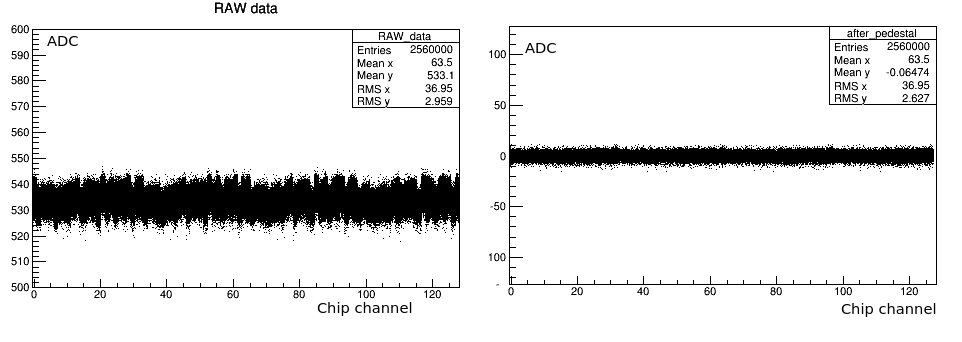
\includegraphics{figures/Pedestal_vs_raw.png}
\caption{Exemplary Pedestal Subtraction Algorithm's monitoring plots. Typical raw data ADC values (left), Pedestal subtracted ADC values
(right).} These plots were generated using data collected during one of the pedestal runs. 
\label{fig:raw vs ped}
\end{figure}


\section{Common mode subtraction}
The next step within the TbUT processing chain is Common mode subtraction and the noise calculation. The determined noise, one floating-point number per channel,  is then used as a clustering threshold value for the clusterization algorithm described in the next section. 


The total noise affecting the signal measurement consist of two main components,  the first one affects every readout channel independently and the second one is common to the group of consecutive channels.  This type of noise is called Common Mode and its origin can be grand loops in the power supplies or readout strips might pick some environmental noise. 

The Common Mode suppression algorithm consists of two phases. The fist one was implemented to calculate the average pedestal-subtracted ADC value of the channels in
32-channel groups. This value is calculated for each event independently. Using this mean value a search for particle hits is performed for each channel. All channels with hits are masked, and a new mean value is calculated for each 32-channel group. The channel is masked when its ADC value fulfills the following condition:

\begin{equation}
    |ADC_{i}(n)-CMS^{corr}_{i}| > \alpha \sigma^{RMS}_{i}
\end{equation}
where $\sigma^{RMS}_{i}$ is a channel ADC Root Mean Square, $CMS^{corr}_{i} $ is a correction for an event $i$, and $\alpha$ is a tunable parameter, that specifies the required distance between noise and signal. After the initial testbeam studies, this parameter was set to 4. 
The previously calculated mean value is then used to correct the ADC values in all channels of the 32-channel group.

The second phase of the CMS algorithm is calculation of the noise per channel, according to the following formula: 

\begin{equation}
    \sigma_i  = \sqrt{\frac{\sum_{n=1}^{N} (ADC_{i}(n)-\mu_{i})^2}{N}}
\end{equation}
where $\mu_{i} = \sum_{n=1}^{N} ADC_{i}(n)$ is a mean ADC value per channel. 


Figure \ref{fig:projections} presents the one-dimensional projection of the data after pedestal and Common Mode subtraction. It is clearly visible, based on the noise values, that the Common mode removal step is necessary to reduce the noise level and thrust increase the Signal-to-Noice (S/N) ratio. 

A few typical events after all corrections applied are shown in figure \ref{fig:Noise}. Here, no requirement is made on the number of tracks. Strips with large ADC counts are indicative of the passage of a beam particle through the detector. The other channels show roughly Gaussian fluctuations about zero, typical of incoherent detector noise. Signals generally
stand out significantly above the noise. These examples were selected to visualize a couple of cases that may occur, such as double strip clusters (event 14) and multiple clusters per event (event 83).  


\begin{figure}[h]
  \centering
\begin{tabular}{c c}
\subfloat{{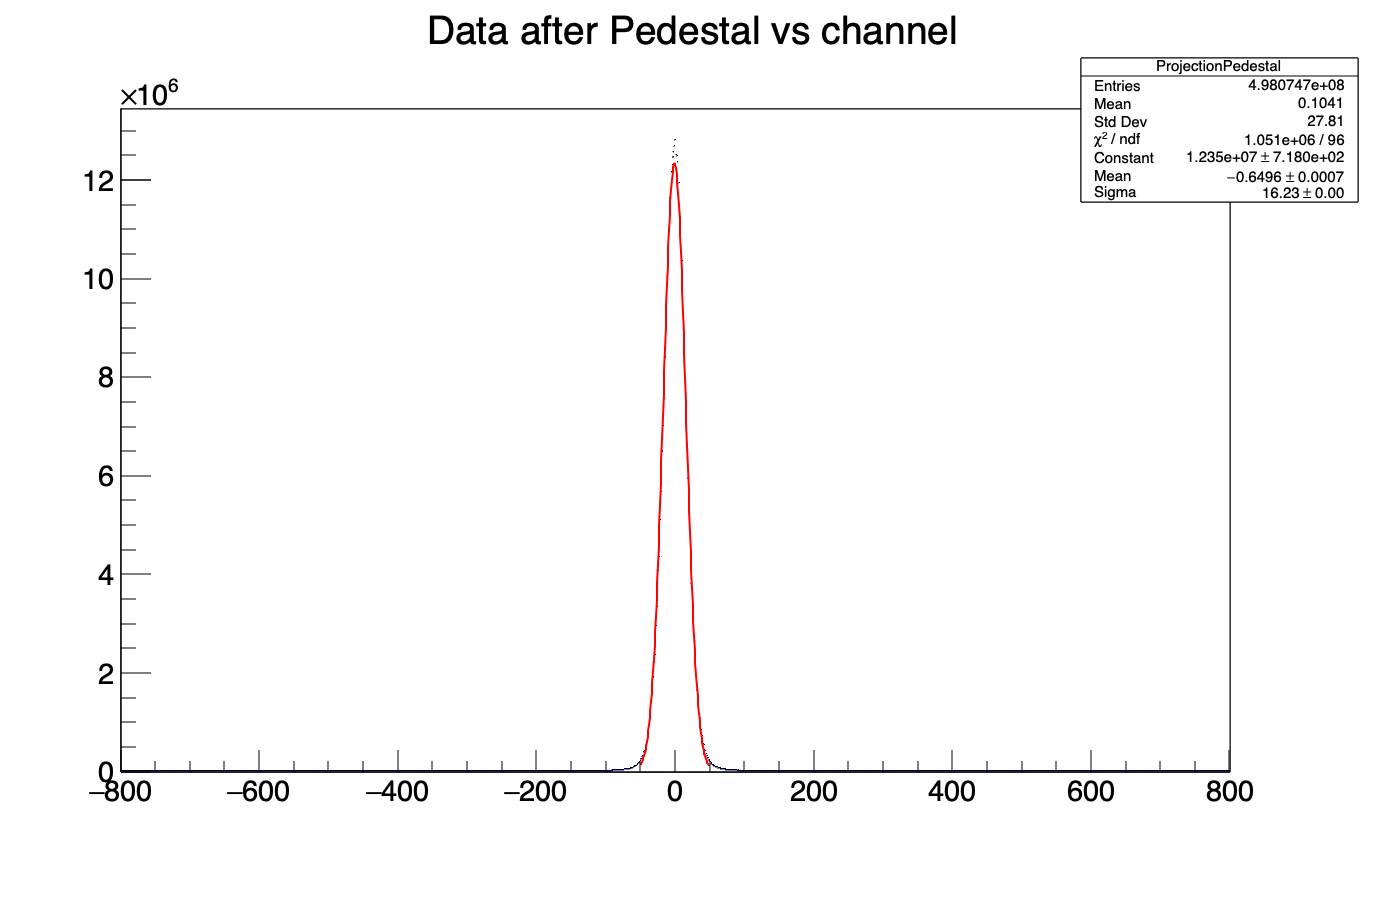
\includegraphics[width=0.5\textwidth]{figures/Pedestal_projection.png} }}%
    \subfloat{{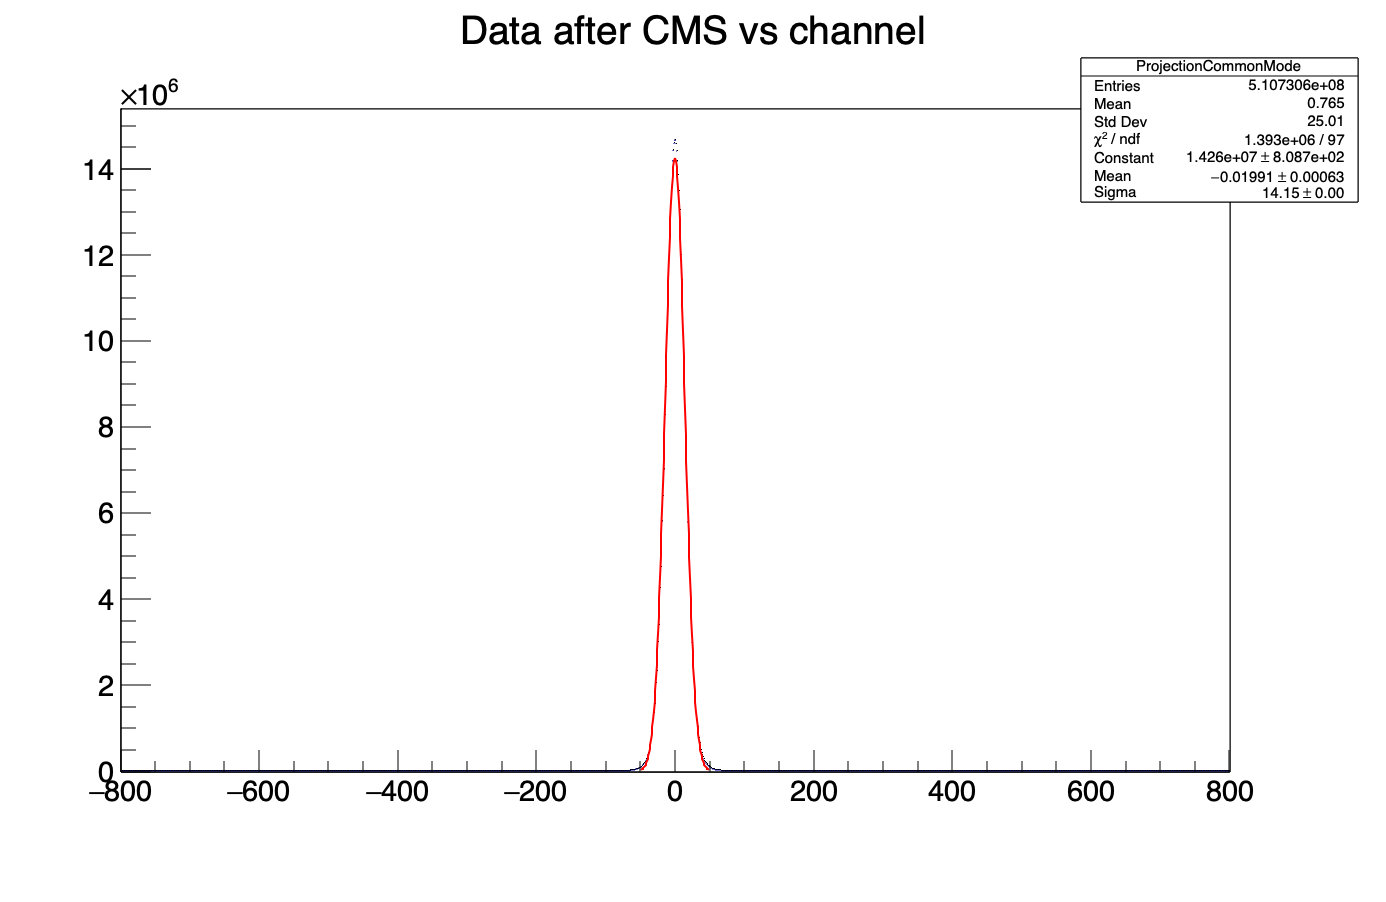
\includegraphics[width=0.5\textwidth]{figures/CMS_projection.png} }}%
\end{tabular}
   \caption{Projection of data after pedestal subtraction (left) and CMS (right)
\label{fig:projections}}  
\end{figure}

\begin{figure}[!h]
  \centering
\begin{tabular}{c c}
\subfloat{{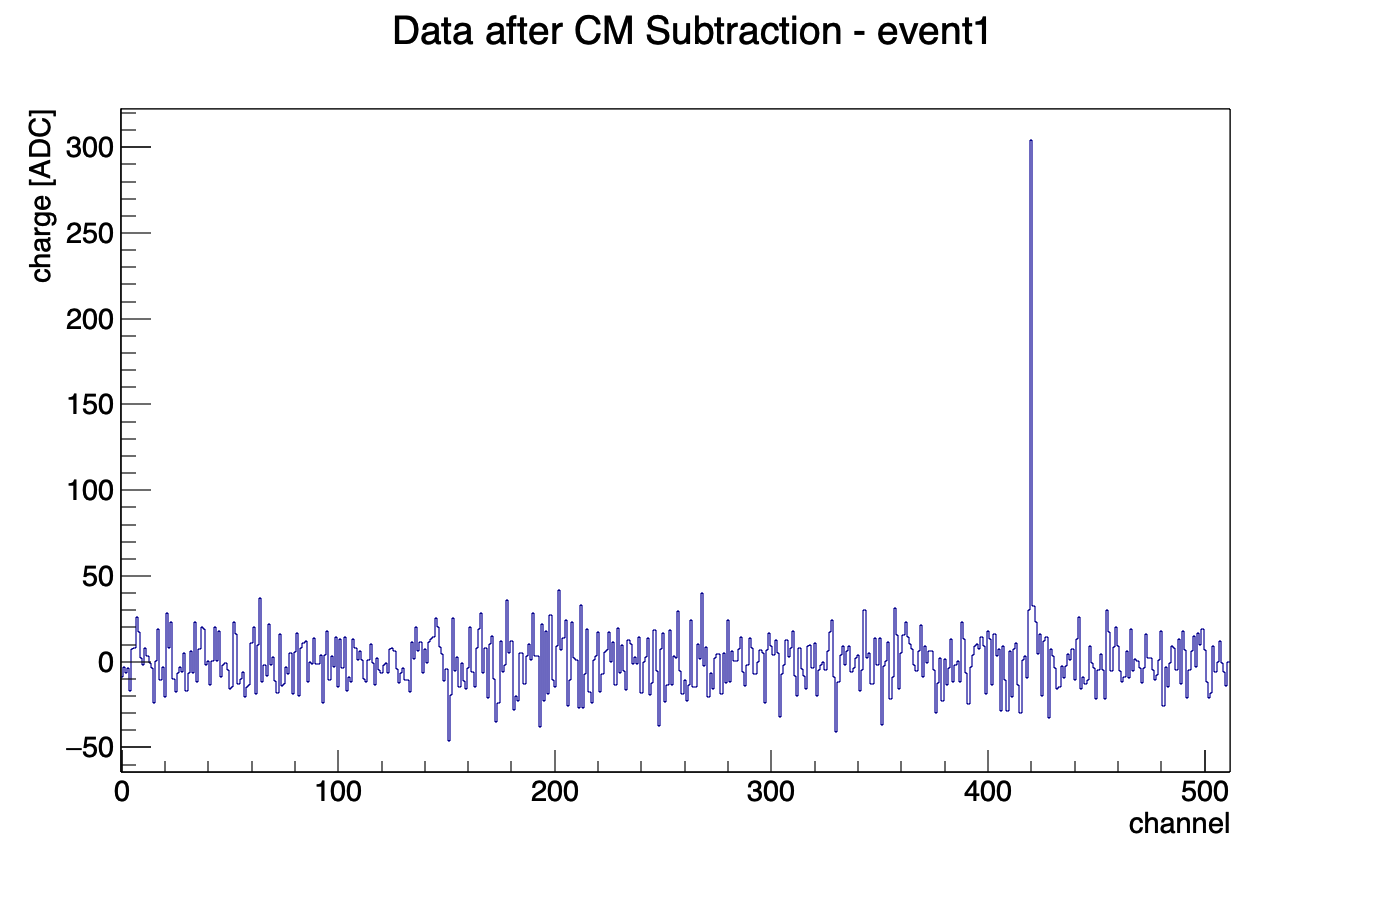
\includegraphics[width=0.5\textwidth]{figures/event1.png} }}%
    \subfloat{{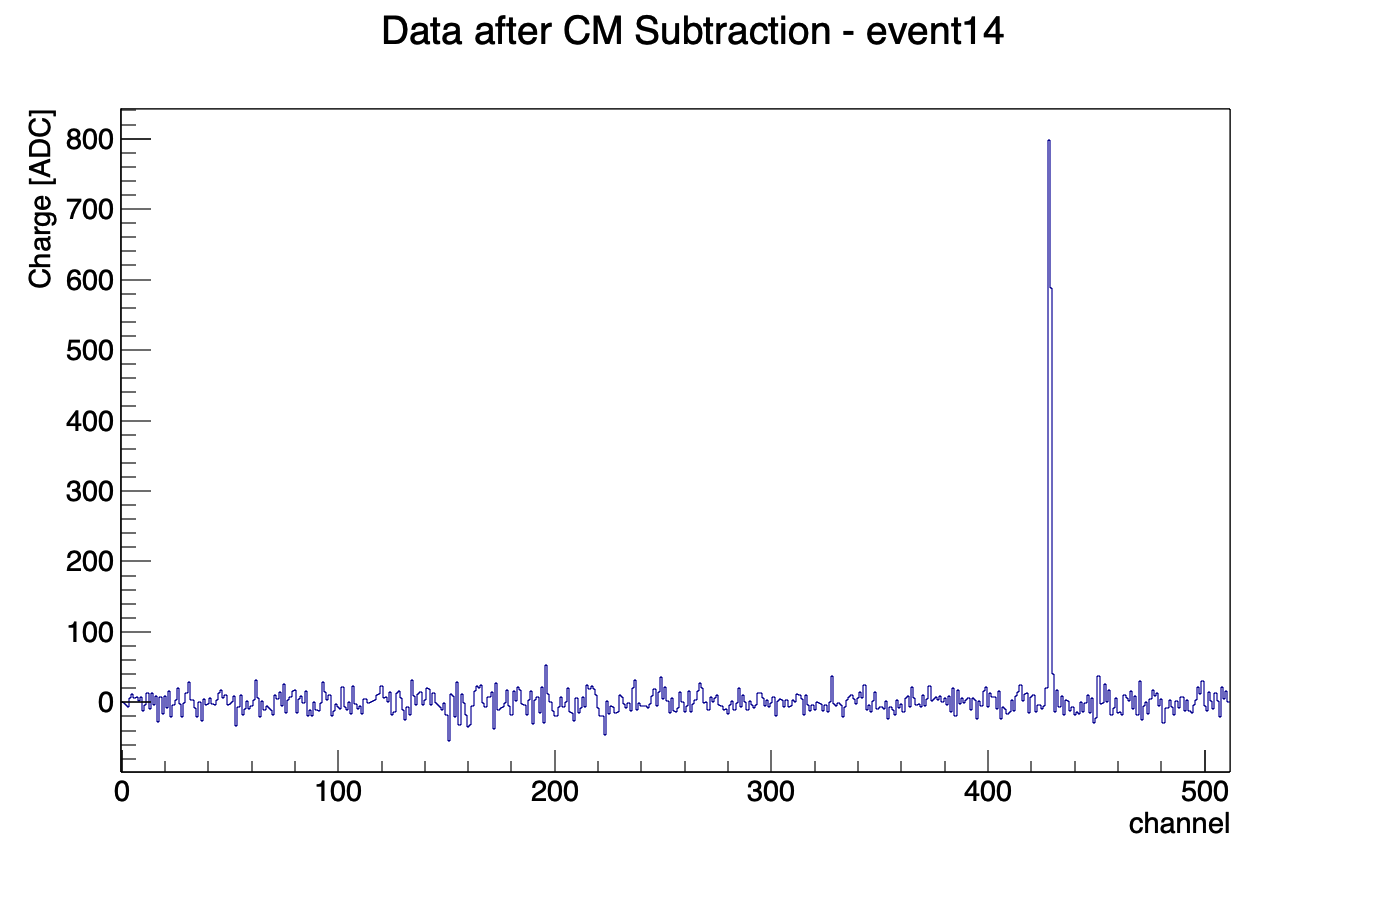
\includegraphics[width=0.5\textwidth]{figures/event2.png} }}%
\\
\subfloat{{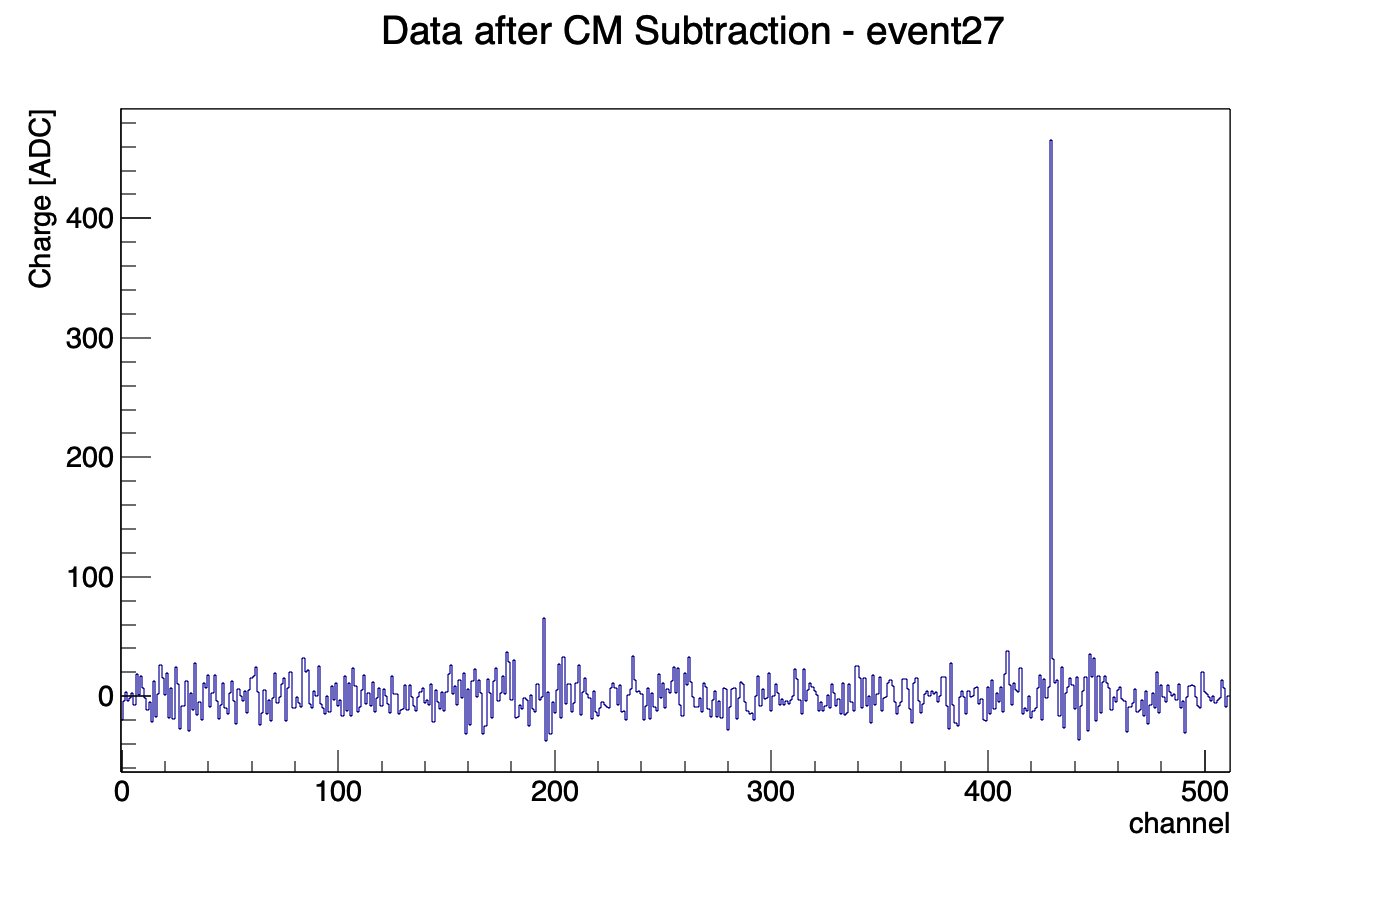
\includegraphics[width=0.5\textwidth]{figures/event3.png} }}%
    \subfloat{{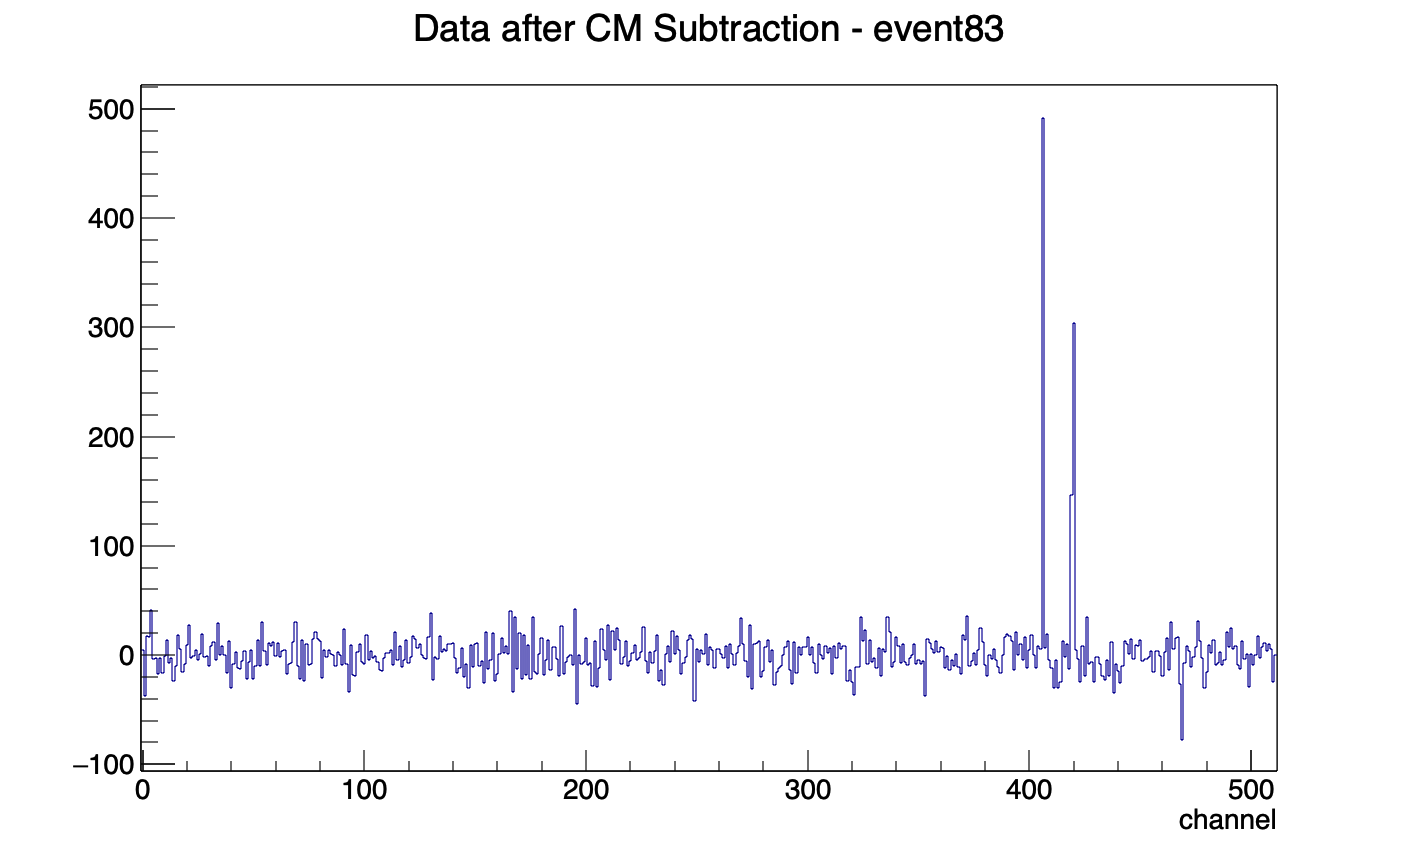
\includegraphics[width=0.5\textwidth]{figures/event4.png} }}%
\\
\subfloat{{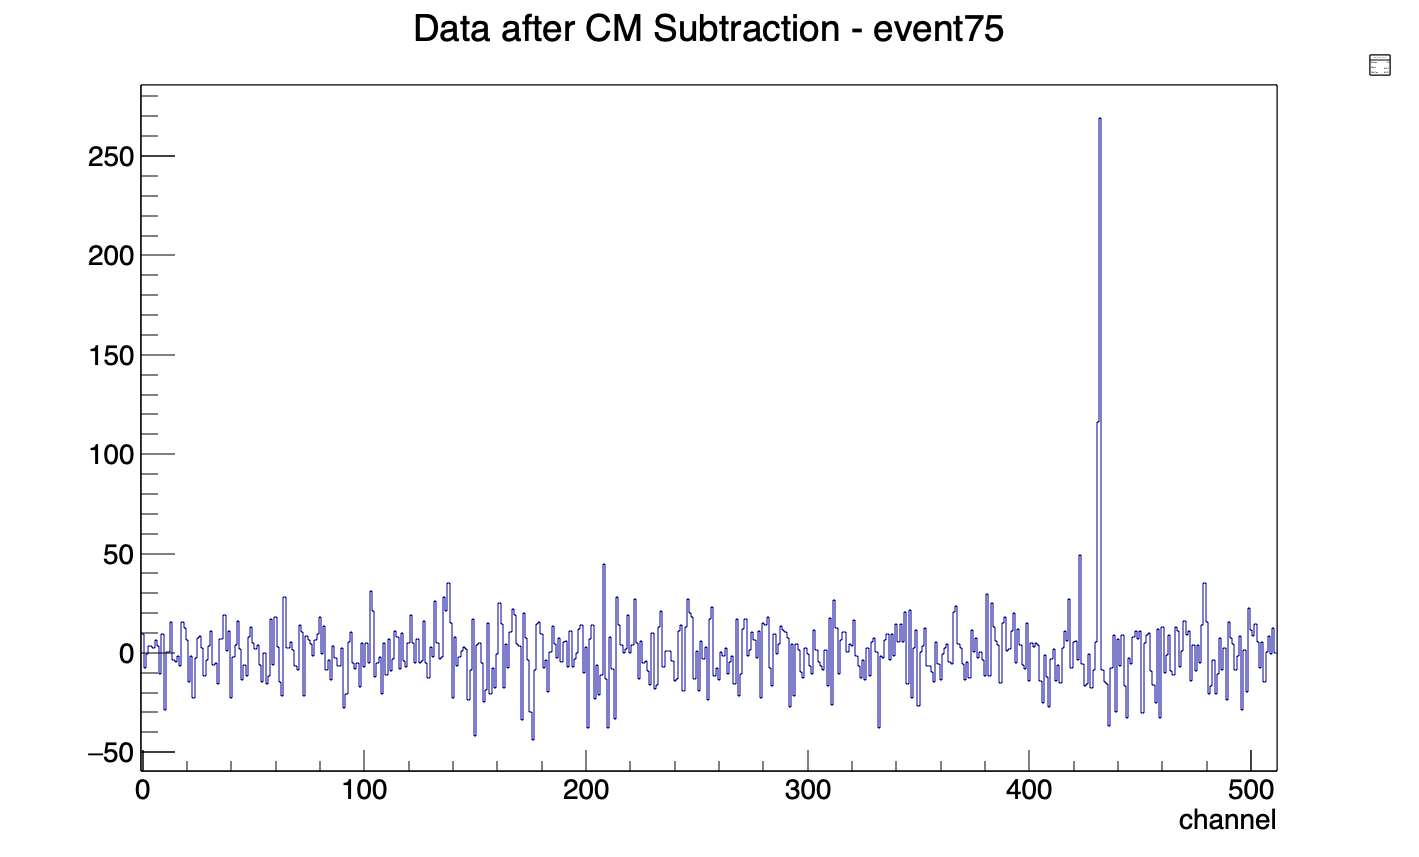
\includegraphics[width=0.5\textwidth]{figures/event5.png} }}%
    \subfloat{{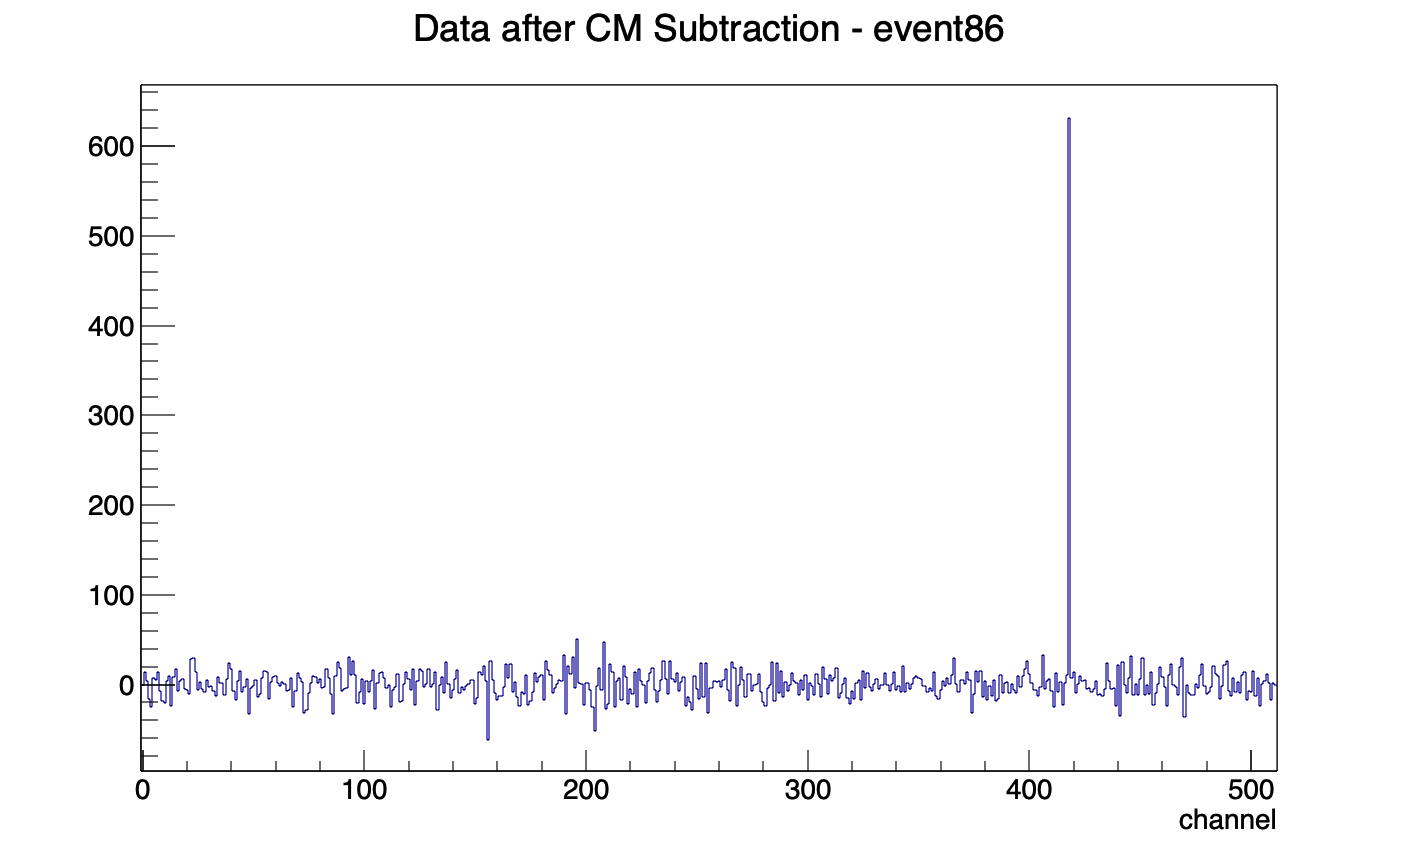
\includegraphics[width=0.5\textwidth]{figures/event6.png} }}%

\end{tabular}
   \caption{A few examples of a single events after pedestal and common mode removal.  
\label{fig:Noise}}  
\end{figure}




\begin{figure}[!h]
  \centering
\begin{tabular}{c c}
\subfloat{{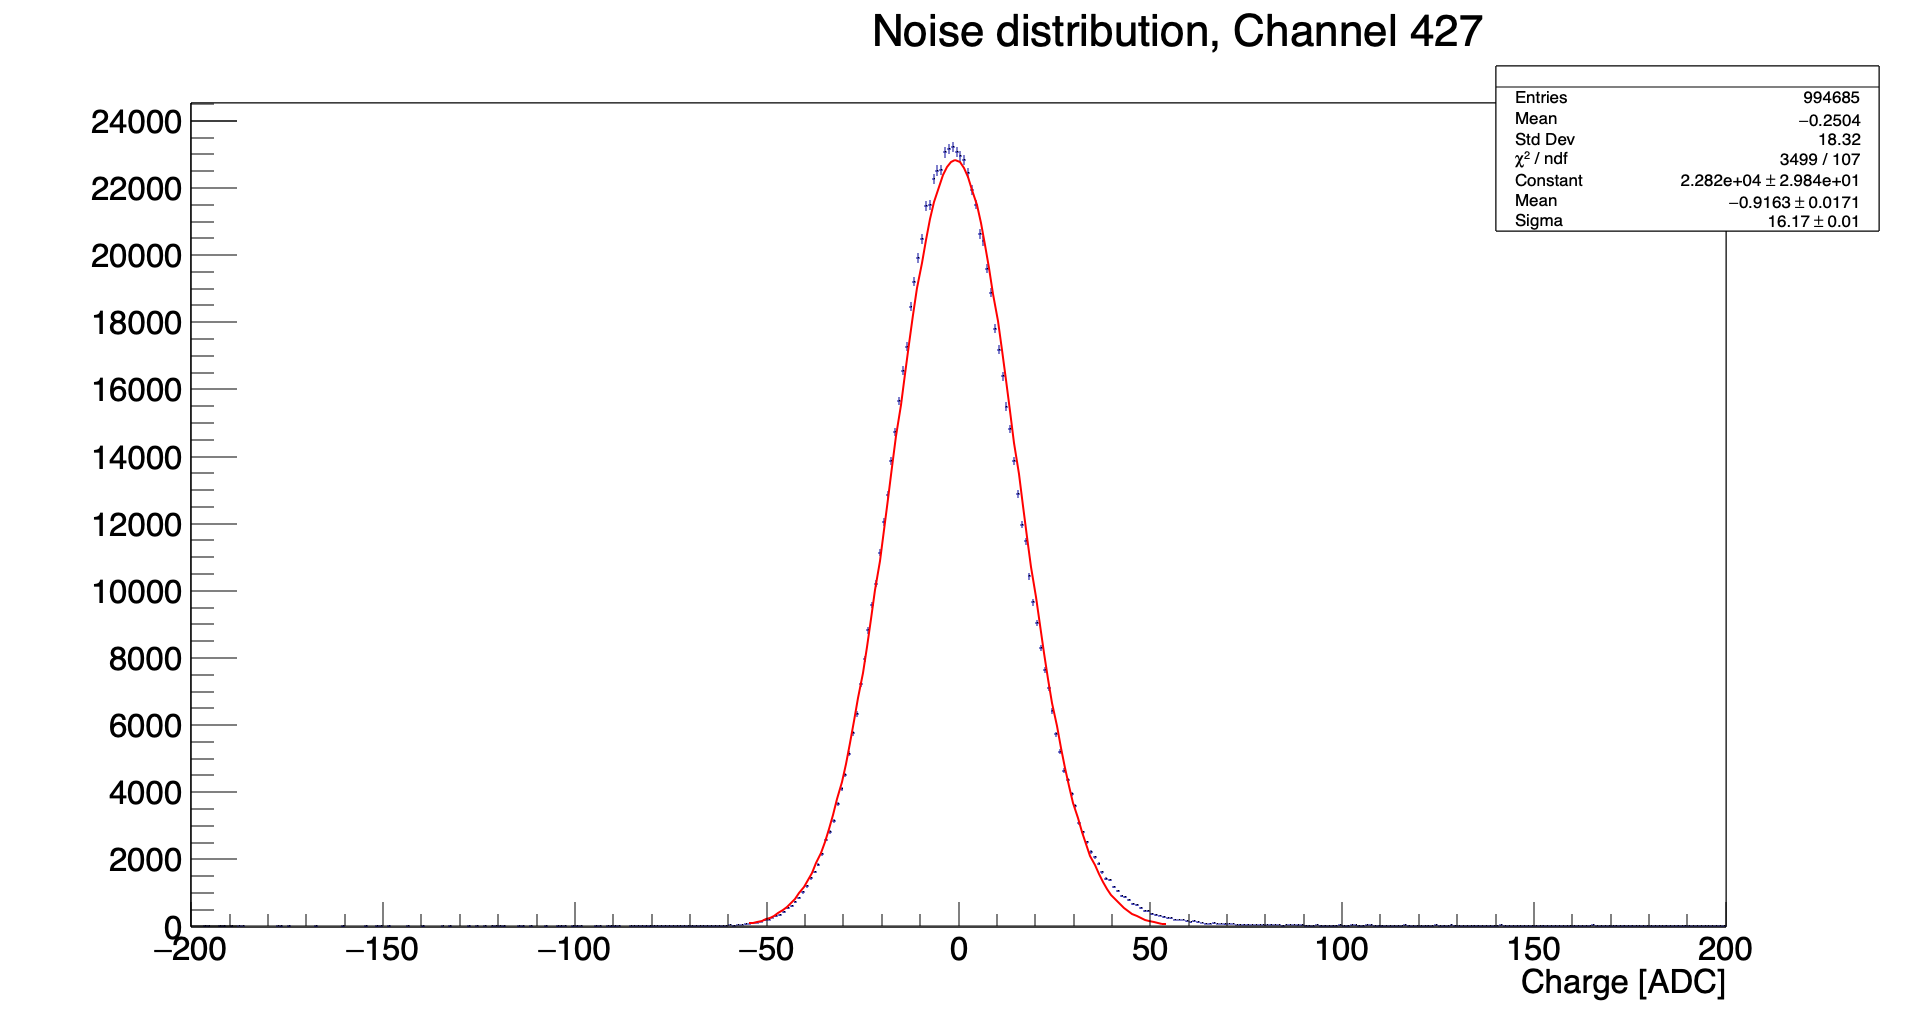
\includegraphics[width=0.5\textwidth]{figures/Noise2.png} }}%
    \subfloat{{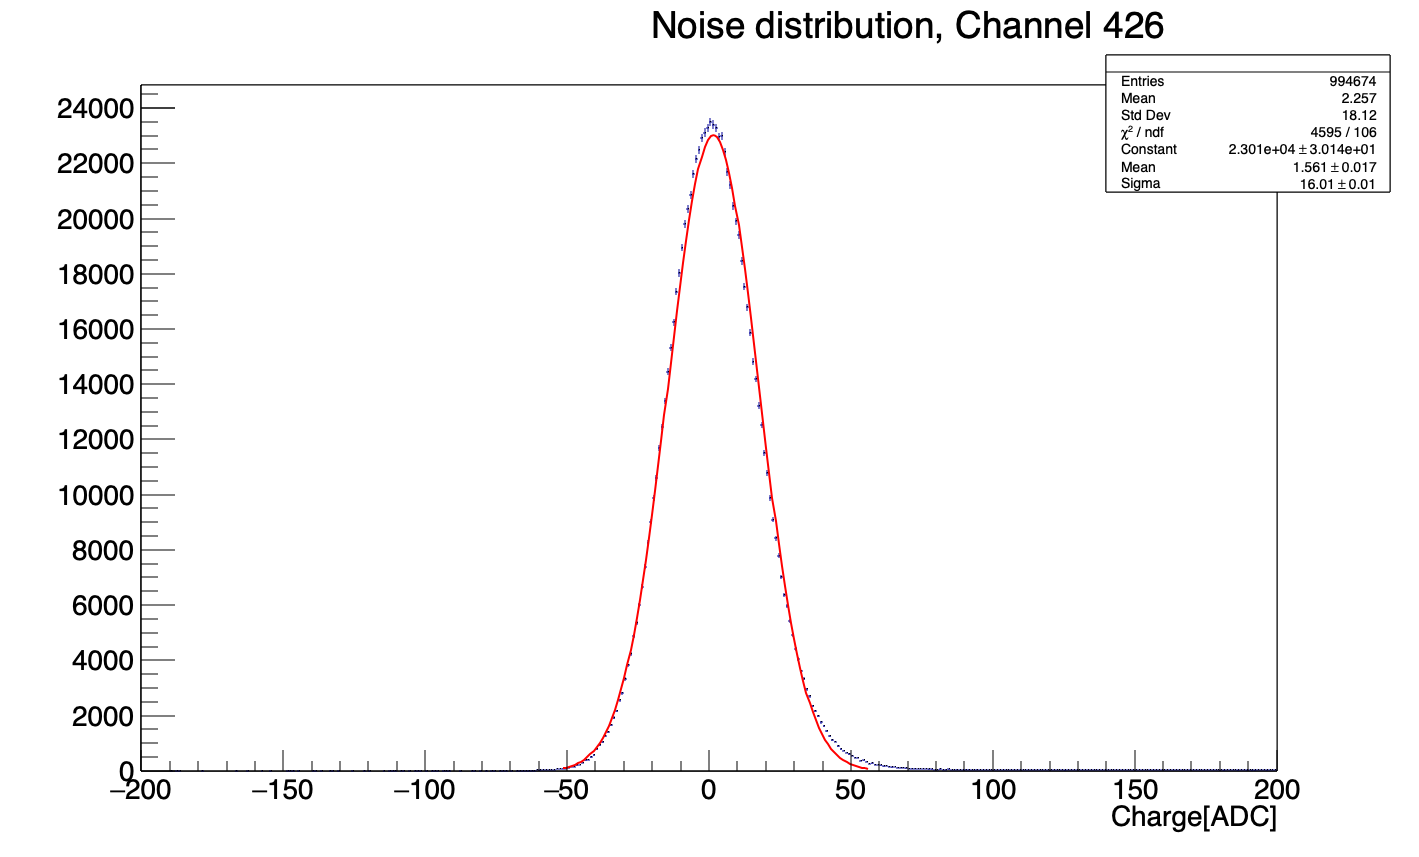
\includegraphics[width=0.5\textwidth]{figures/Noise0.png} }}%
\\
\subfloat{{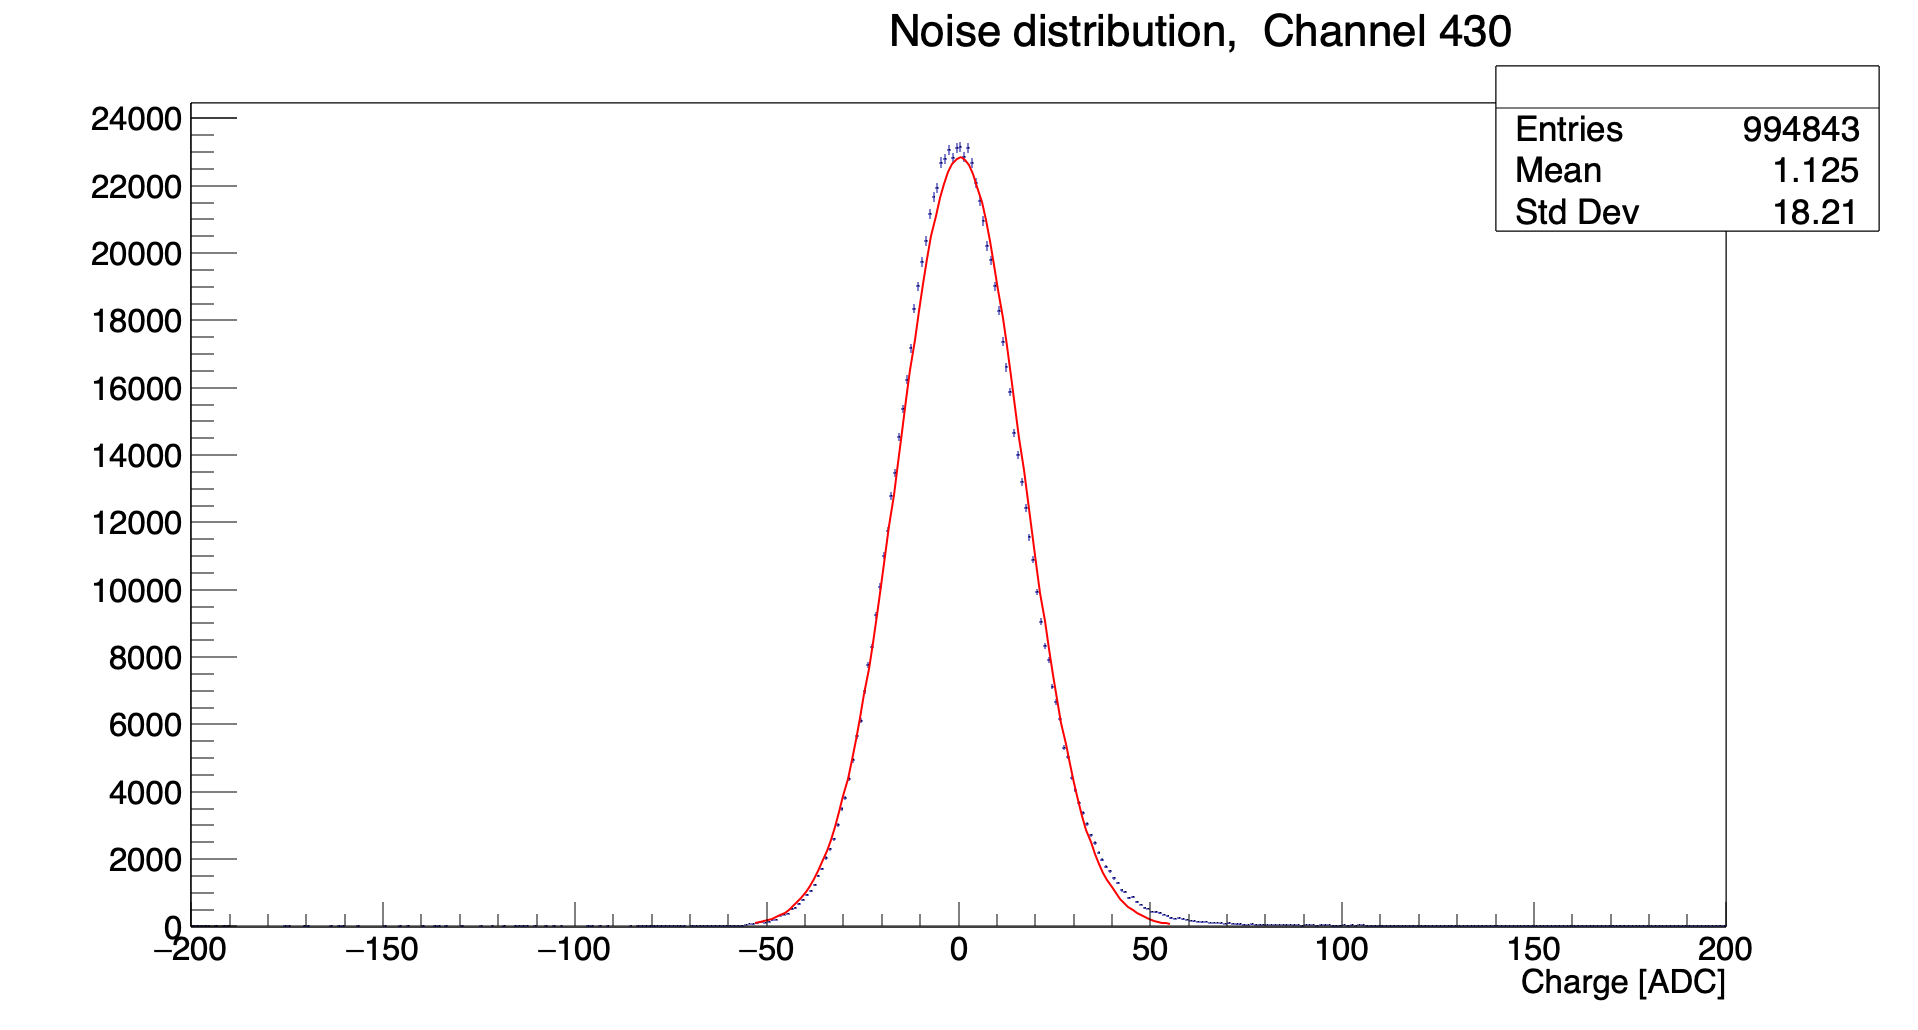
\includegraphics[width=0.5\textwidth]{figures/Noise3.png} }}%
    \subfloat{{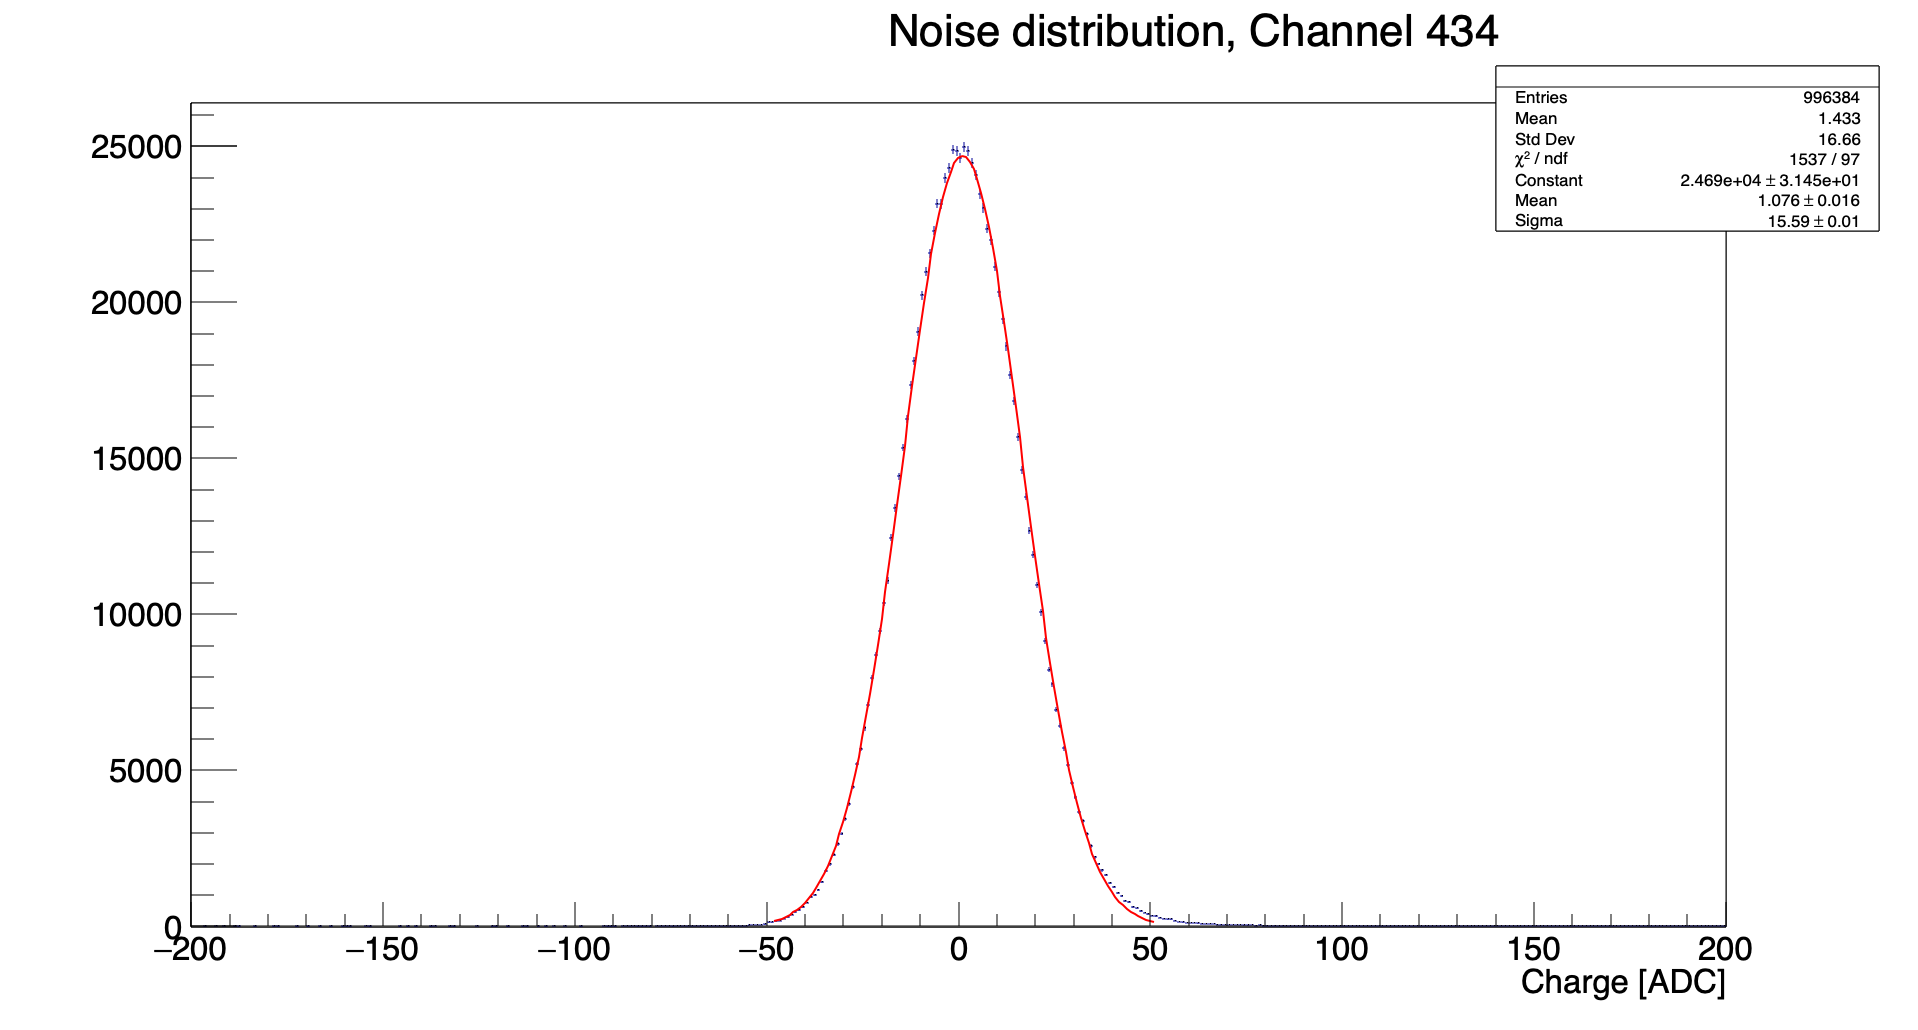
\includegraphics[width=0.5\textwidth]{figures/Noise4.png} }}%
\\
\subfloat{{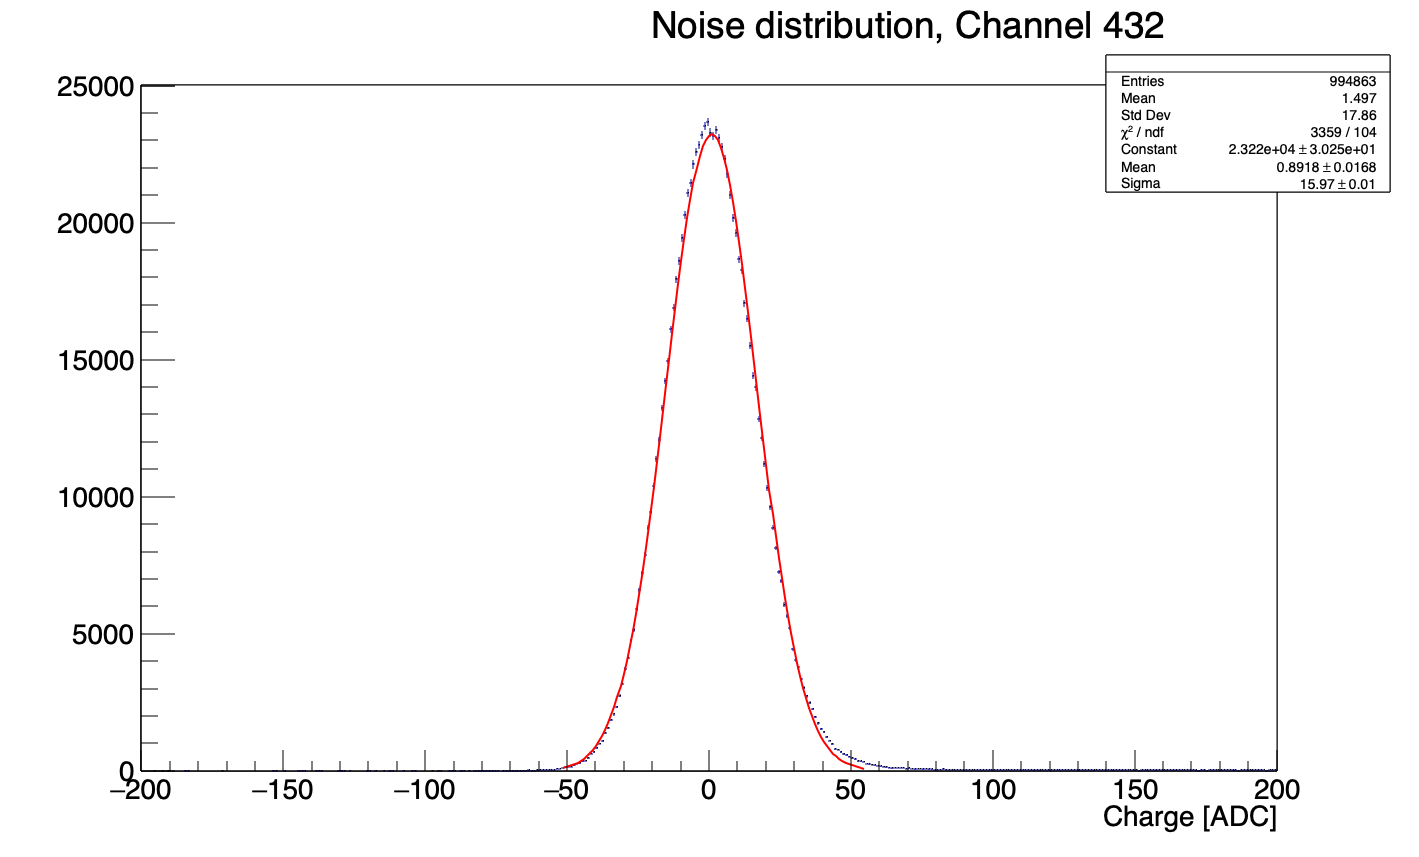
\includegraphics[width=0.5\textwidth]{figures/Noise5.png} }}%
    \subfloat{{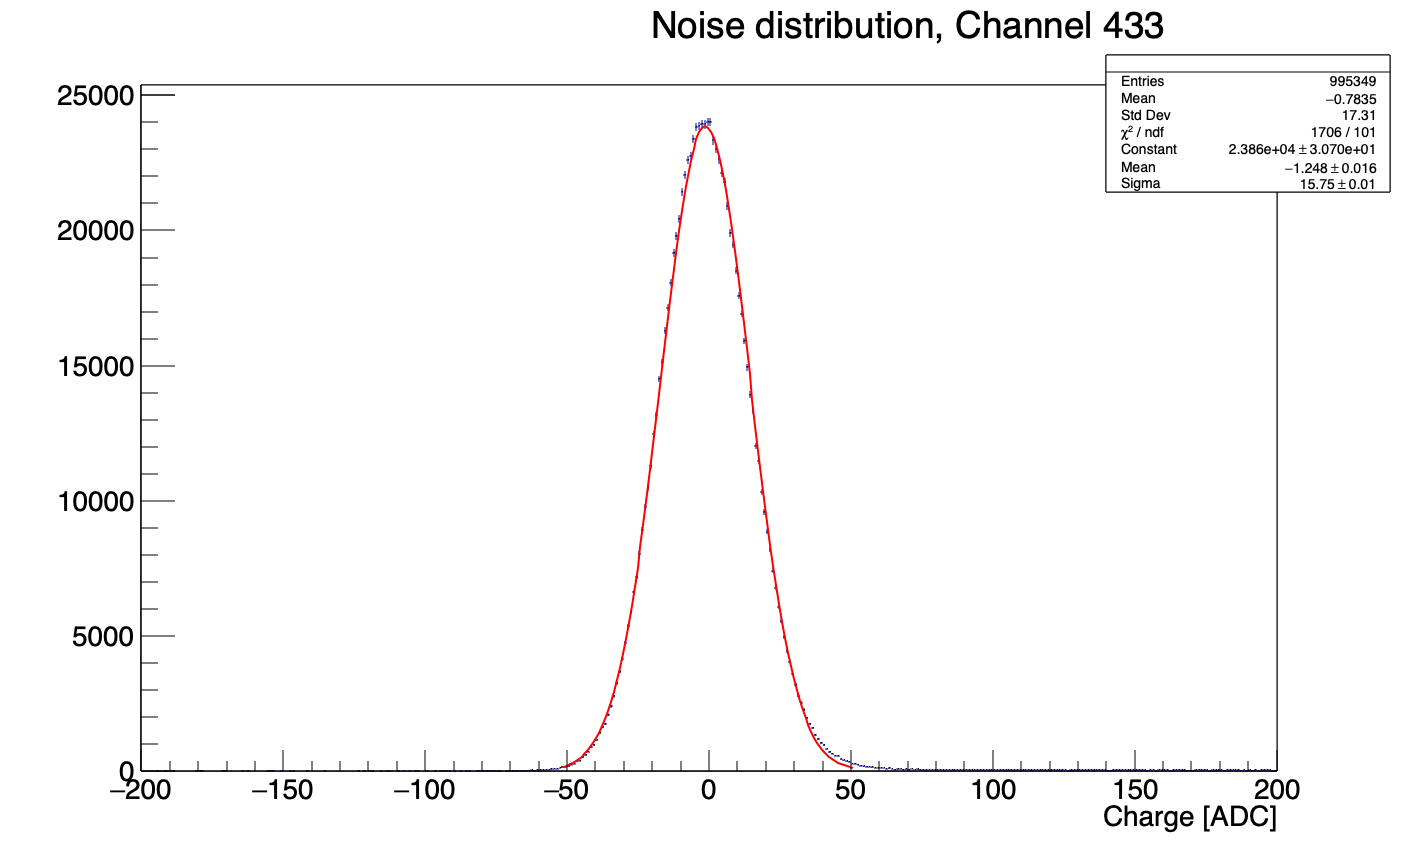
\includegraphics[width=0.5\textwidth]{figures/Noise6.png} }}%

\end{tabular}
   \caption{Noise distributions after Common Mode Suppression for selected channels within the beam region. The red curves show a Gaussian fit to the core of the distribution. 
\label{fig:Noise}}  
\end{figure}


\section{Cluster finding algorithm}

The final algorithm is executed to reconstruct a cluster using previously proceeded ADC values and noise per channel, which plays the role of the clusterization threshold.  
The additional algorithm’s input parameters are the value of the low and high thresholds. 
Clusters in the DUT are built up by searching for a seed strip that has a collected charge more than a high threshold value. The outcome of this subroutine is a list of cluster seeds. The next subroutine is dedicated to removing the seeds that belong to the same clusters. Such a situation occurs when the cluster has more than one strip and all of them have collected charges value higher than the high threshold. 
Moving away from the seed strip, the adjacent side strips having at least ADC count as low threshold, are added to the cluster seed. The cluster is terminated when a side strip charge is below a low threshold. Thus, by definition, a cluster has between 1 and 5 strips included.
When there are multiple strips in the cluster, the position is computed using linear charge weighting:

\begin{equation}
    x_{cluster} = \frac{\sum^{S}_{i=1}x_i q_i}{{\sum_{i=1}{S}{q_i}}}
\end{equation}
where $x_i$ and $q_i$ are the positions and charges of
the strips in the cluster, and $S$ is the number of strips that constitute the cluster. 
\begin{algorithm}[caption={cluster creator algorithm}, label={al:cluster creator}]
Data: ADC data after Common Mode Suppression ($1 \ldots N$ events), clusterization thresholds (one floating point number per channel)
Result: vector of reconstructed clusters

for event in $1 \ldots N$ do :
   find cluster seeds;
   remove seeds belonging to the same clusters;
   extend cluster seeds by adding adjacent strips;
   calculate cluster position
end
\end{algorithm}


The outcome of the clusterization algorithm can be visualized in a couple of different ways. One of the most popular is the plot that presents the distribution of the cluster charge. To get an important physics quantities describing the performance of the sensor the data is fitted to the Landau Gauss convolution model, see section \ref{sec:Interaction}:


\begin{figure}
\begin{subfigure}
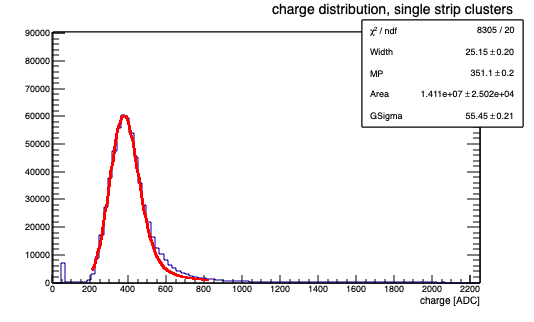
\includegraphics{figures/single_strip.png}
\end{subfigure}
\hfill
\begin{subfigure}
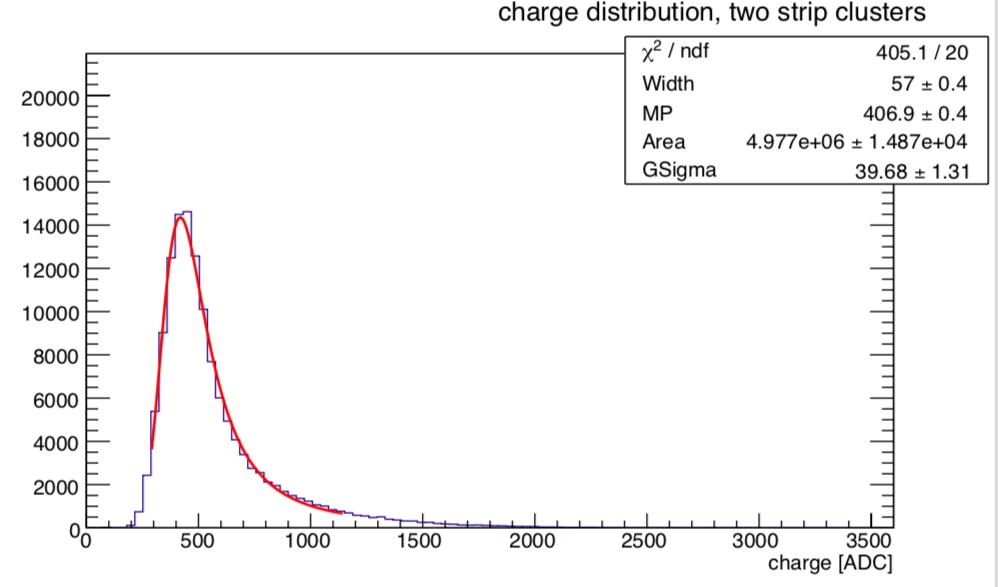
\includegraphics{figures/two_strip_charge.png}
\end{subfigure}%
\caption{Cluster charge distributions. The upper plot presents charge distribution for 1-strip clusters and the bottom one for 2-strip clusters . The data are fit to a Landau
convoluted with a Gaussian resolution function, and the fit is shown (red solid line).
}\label{fig:limeResult}
\end{figure}
